%----------------------------------------------------------------------------------------
%	PACKAGES AND DOCUMENT CONFIGURATIONS
%----------------------------------------------------------------------------------------

\documentclass{article}

\usepackage[version=3]{mhchem} % Package for chemical equation typesetting
\usepackage{siunitx} % Provides the \SI{}{} and \si{} command for typesetting SI units
\usepackage{graphicx} % Required for the inclusion of images
\usepackage{natbib} % Required to change bibliography style to APA
\usepackage{amsmath} % Required for some math elements 
\usepackage[utf8x]{inputenc} 
\usepackage{booktabs}
\usepackage{tabto}
\usepackage{amssymb}
\usepackage{listings}
\usepackage{float}
\restylefloat{figure}


\renewcommand{\labelenumi}{\alph{enumi}.} % Make numbering in the enumerate environment by letter rather than number (e.g. section 6)

%----------------------------------------------------------------------------------------
%	DOCUMENT INFORMATION
%----------------------------------------------------------------------------------------

\title{Tema 3} % Title

\author{Shanti \textsc{Zmuschi} și Andrei \textsc{Ianău}} % Author name

\date{10/01/2020}

\begin{document}

\maketitle % Insert the title, author and date

\begin{center}
\begin{tabular}{l r}
Profesor: &  Olariu E. Florentin \\ % Instructor/supervisor
\end{tabular}
\end{center}



%----------------------------------------------------------------------------------------
%	Problema 1
%----------------------------------------------------------------------------------------

\section*{Problema 1}
Presupun ca exista un e-flux fezabil, asta inseamna ca exista $x:E \rightarrow \mathbb{R}$ astfel incat \\
$$ 0 \leq x_{ij} \leq c_{ij}, \forall ij \in E$$
$$ \sum_{j}x_{ij} = \sum_{j}x_{ji} \forall i \in V-(X \cup Y) $$
$$ \sum_{j}x_{ij} -  \sum_{j}x_{ji}  \leq \sigma_i \forall i \in X \Rightarrow \sum_{j}x_{ij} \leq \sum_{j}x_{ji}  + \sigma_i \forall i \in X (1) $$
$$ \sum_{j}x_{ij} -  \sum_{j}x_{ji}  \leq \theta_i \forall i \in Y \Rightarrow \sum_{j}x_{ij} \leq \sum_{j}x_{ji}  + \theta_i \forall i \in Y (2) $$  
Consideram doua multimi aleatoriu alese: S si T astfel incat $S\cup T = V \land S \cap T = \emptyset$
$$(1)\land (3) \Rightarrow  \sum_{ji \in E; i \in X\cap T}x_{ji} \geq \sum_{ij \in E; i \in X\cap T}x_{ij} - \sum_{i \in X\cap T}\sigma_i $$ 
$$(2)\land (3) \Rightarrow  \sum_{ji \in E; i \in Y\cap S}x_{ji} \geq \sum_{ij \in E; i \in Y\cap S}x_{ij} - \sum_{i \in Y\cap S}\theta_i $$ 
Din cele doua anterioare rezulta:
$$ \sum_{ji \in E; j \in Y\cap S; i \in X\cap T}x_{ji} \geq  \sum_{i \in Y\cap S}\theta_i - \sum_{i \in X\cap T}\sigma_i +  \sum_{ij \in E; j \in Y\cap S; i \in X\cap T}x_{ij}$$ 
Inseamna ca 
$$ x_{ij} \geq 0, \forall ij \in E \Rightarrow 2  \sum_{ij \in E; j \in Y\cap S; i \in X\cap T}x_{ij} \geq 0$$
$$\Rightarrow \sum_{ij \in E; j \in Y\cap S; i \in X\cap T}x_{ij} \geq \sum_{i \in Y\cap S}\theta_i - \sum_{i \in X\cap T}\sigma_i   $$
$$ ji \in E \Rightarrow \sum_{ji \in E}{x_ji} \leq \sum{ji \in E}{c_ji} $$
Din cele doua anterioare rezulta:
$$ \sum_{ji \in E; j \in Y\cap S; i \in X\cap T}c_{ji} \geq  \sum_{i \in Y\cap S}\theta_i - \sum_{i \in X\cap T}\sigma_i +  \sum_{ij \in E; j \in Y\cap S; i \in X\cap T}x_{ij}$$ 
$$ c_{ij} \geq 0, \forall ij \in E \Rightarrow  \sum_{ji \in E; j \in  S; i \in T}c_{ji} \geq \sum_{ji \in E; j \in Y\cap S; i \in X\cap T}c_{ji} $$
Din cele doua anterioare rezulta:
$$ \sum_{ji \in E; j \in  S; i \in T}c_{ji} \geq \sum_{i \in Y\cap S}\theta_i -  \sum_{i \in X\cap T}\sigma_i $$



%----------------------------------------------------------------------------------------
%	Problema 2
%----------------------------------------------------------------------------------------

\section*{Problema 2}

(a)(b)
\begin{figure}[H]
  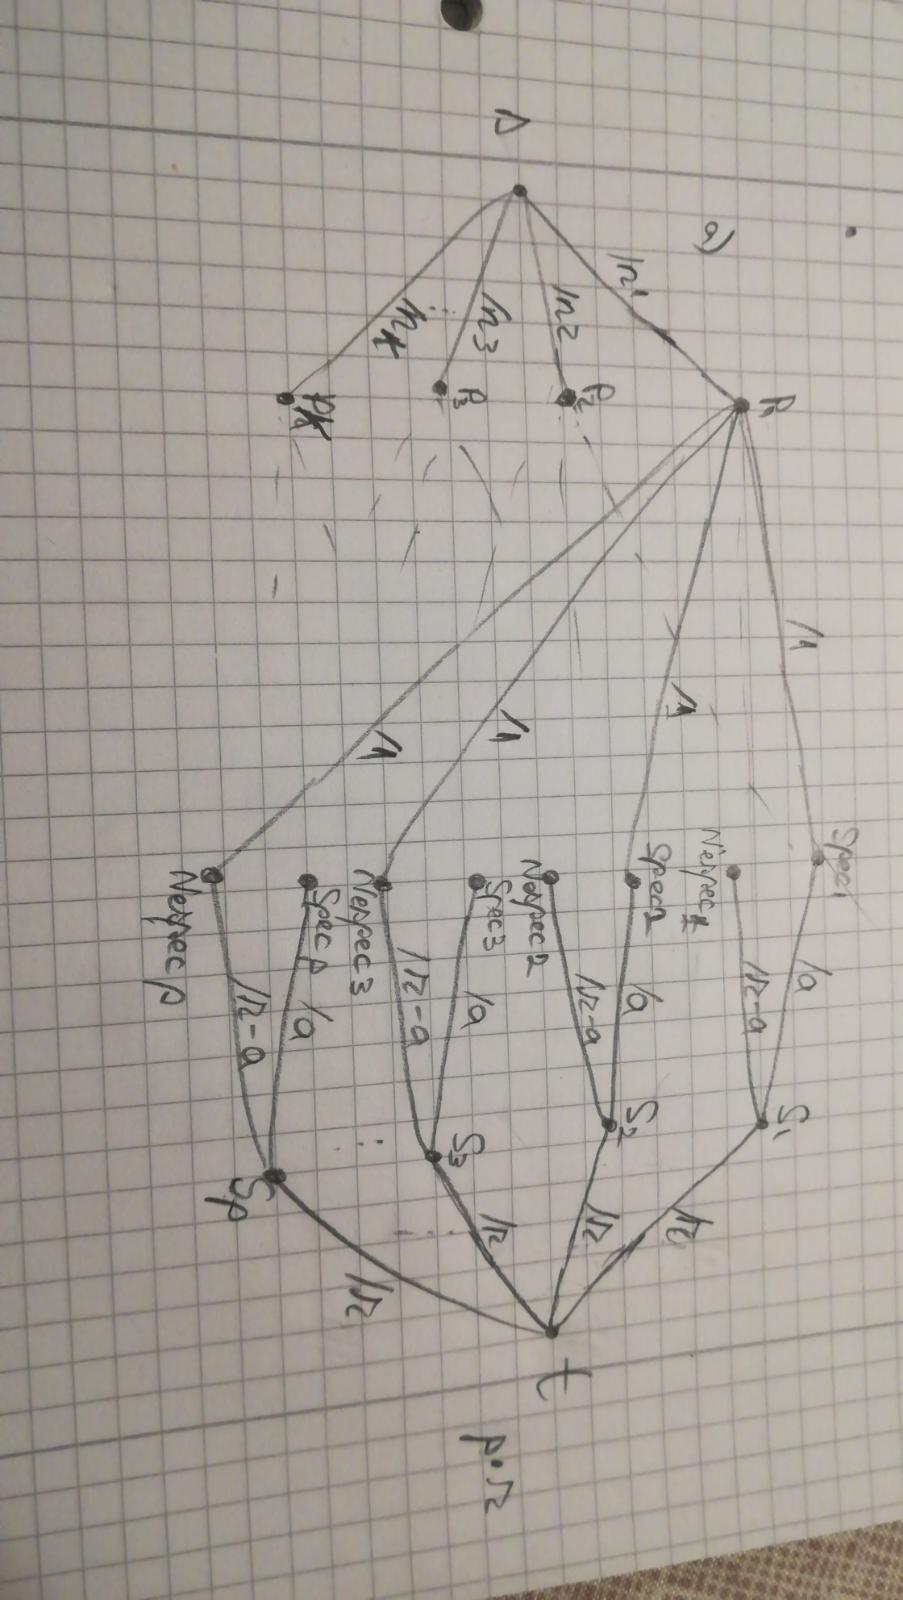
\includegraphics[width=60mm]{2a.jpeg}
 \end{figure}

Modelam reteaua astfel (ca in poza). O unitate de flux inseamna ca un profesor va judeca o lucrare de licenta (muchie  $s \rightarrow P_i$). Toate muchiile    $s \rightarrow P_i$ au capacitatea maxima $n_i$ (adica poate participa maxim la  $n_i$ prezentari). Apoi, din acesta vor iesi muchii catre $Spec_i$, $Nespec_i$ daca acesta este specializat sa judece licenta studentului i, respectiv nu este specializat. Aceste muchii vor avea capacitatea 1 (adica va fi sau nu prezent la prezentare). Fiecare nod $Spec_i$, $Nespec_i$ va avea muchie catre un $S_i$ cu o capacitate de $a$ (adica cei specializati vor fi in numar de $a$), respectiv $r-a$  (adica cei specializati vor fi in numar de $r-a$). Astfel fiecare student $S_i$ va avea muchie cu $t$ de capacitate $r$, ceea ce inseamna ca daca in total, fluxul maxim in $t$ este $pr$, unde $p$ este numarul de studenti, inseamna ca prezentarea licentelor poate avea loc.
(c)
 Folosind  algoritmul Edmonds-Karp vom avea o complexitate de $O(VE^2)$  



%----------------------------------------------------------------------------------------
%	Problema 3
%----------------------------------------------------------------------------------------

\section*{Problema 3}

\begin{figure}[H]
 	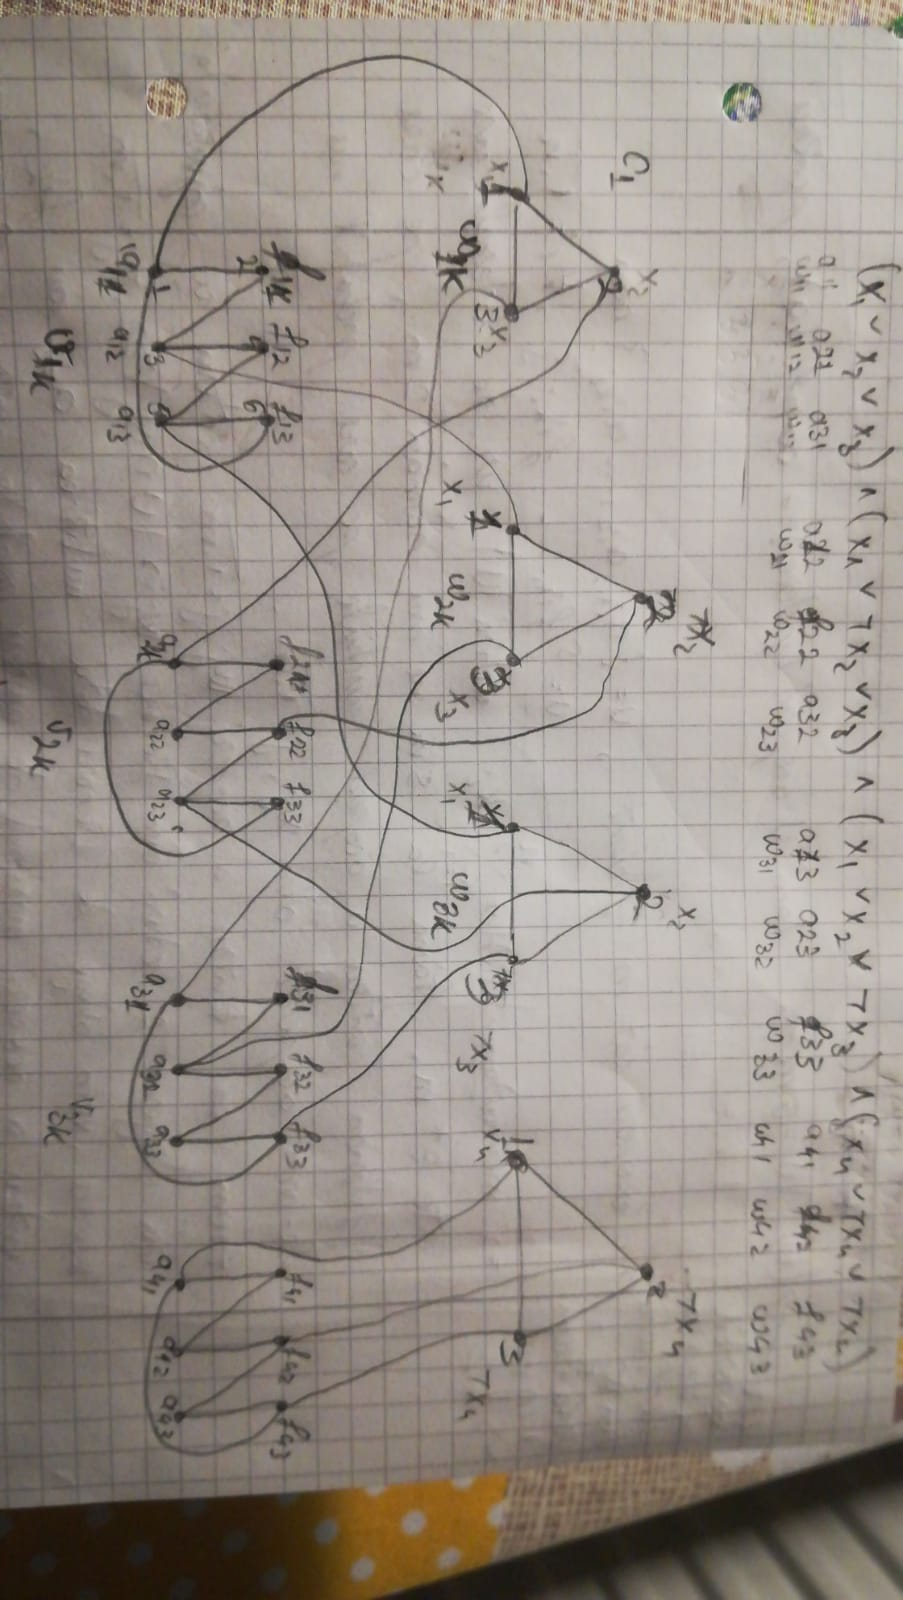
\includegraphics[width=60mm]{3.jpeg}
\end{figure}

Datorita definitiei lui $G_i, \forall v \in V(G_i), v_j = 
  \begin{cases}
	a_{ij}, & \text{daca } j \%2 =0, \\
  	f_{ij}, & \text{altfel}.
  \end{cases}
$
j fiind index a lui v, numerotand de la $a_{i1}$. Astfel pentru a putea acoperi toate muchiile cu o multime de cardinal minim tb sa alegem nodurile de pe pozitii pare sau impare, astfel formandu-se chiar multimile ${a_{i1}, ... a_{ik_i}}$ sau ${f_{i1}, ... f_{ik_i}}$

(b1) Este imposibil sa acoperim cele 3 muchii din $W_j , \forall j = 1...m$ daca luam
un singur nod. Astfel pentru a acoperi toate muchiile trebuie sa luam minim 2
noduri. qed.

(b2) Cum multimea U acopera (din ipoteza), inseamna ca conform (a), pentru a acoperi
cat mai eficient, $\bigcup_{i=1}^{n}{\{a_{i,l}|l=1...k_i\}}$ , astfel vom avea $|U| = \sum_{i=1}^{n}{k_i}$.
Adica cardinal de U este numarul de literali, care este de fapt $3m$. Cum acesta este
cel mai bun caz (adica minimul), putem luat oricate noduri din $V_i$ astfel incat
$|U \cap (\bigcup_{i=1}^{n}{V_i})| \geq 3m$

(b3) Din punctele precedente: pt a acoperi muchiile lui $V_i \forall i = 1...n$, vom
alege sau $\{a_{i1}, ... a_{ik_i}\}$ sau $\{f_{i1}, ... f_{ik_i}\}$. Avem 
$|U| = \sum_{i=1}^{n}{k_i} = 3m $
momentan. Pentru a acoperi si restul muchiilor neacoperite, vom alege din
nodurile fiecarui $W_j$ si vom alege cate doua dintre nodurile care au 3 muchii
care au 3 muchii neacoperite. Atfel vom avea 
$|U| = \sum_{i=1}^{n}{k_i} + \sum_{i=1}^{m}{2} = 3m + 2m = 5m$.

(b4) $\Rightarrow $Din definitiile multimilor A si F vom avea ca daca toate aparitiile lui
$x_i$ sunt ne-negate (astfel avand evaluate clauzele in care se regasesc la adevarat),
vom avea faptul ca vom alege multimea ${a_{i1}, ... a_{ik_i}}$  pentru a putea acoperi
G cu U, $|U| = 5m$ (conform punctelor anterioare). $\Leftarrow$ Deoarece am ales $U \cap V_i =
{a_{i1}, ... a_{ik_i}}$, inseamna ca toate aparitiile literlului $x_i$ sunt pozitive, ceea ce
face ca asignarea $t(x_i) = true$ sa faca clauza in care apare $x_i$ sa fie evaluata la
adevarat

%----------------------------------------------------------------------------------------
%	Problema 4
%----------------------------------------------------------------------------------------

\section*{Problema 4}

(a)
 Conform spuselor din curs, daca aplicam algoritmul de colorare greedy, vom avea clase de de clolorare optimale $\{S_i | i=1...\chi(G)\}$  astfel incat cel putin una dintre $S_i$ este o multime stabila maximala. (curs agr11.pdf) 

(b) $\chi(G) ≤ \chi(G + xy)$. De asemenea, daca luam ın considerare o colorare
de $G|xy$ cu $\chi(G|xy)$ culori, atunci putem colora graful G prin colorarea x si y
aceeasi culoare ca $(x, y)$ contractat si coloram totul la fel. Deci $\chi(G) ≤ \chi(G|xy)$.
Acum daca $\chi(G) < \chi(G + xy)$, stim ca fiecare colorare de G folosind $\chi(G)$
culori trebuie sa aiba x si y colorate la fel. In caz contrar, am putea folosi aceeasi
colorare pentru $G + xy$.
Alegem o colorare de G cu culori $\chi(G)$. Atunci pentru graficul $G|xy$, trebuie
sa luam ın considerare exact aceeasi colorare, unde fiecare $v \neq x, y$ este colorat
la fel ca ın G, iar nodul contractat $(x, y)$ are aceeasi culoare ca x si
y(deoarece x si y au aceeasi culoare).
Asta inseamna ca daca $\chi(G) < \chi(G + xy)$, atunci $\chi(G) = \chi(G|xy)$.


\end{document}